\documentclass[12pt,oneside,letterpaper]{article}

\usepackage[canadien]{babel}
\usepackage[utf8]{inputenc}
\usepackage[T1]{fontenc}
\usepackage{lmodern}
\usepackage{graphicx}
\usepackage[letterpaper]{geometry}
\usepackage[americanvoltages,americancurrents, siunitx]{circuitikz}
\usetikzlibrary{babel}
\usepackage{amsmath}
\usepackage{caption}
\usepackage{subfig}
\usepackage{hyperref}
\usepackage[all]{hypcap}
\usepackage{multirow}


\captionsetup{font=small,labelfont=bf,margin=0.1\textwidth}
\pagestyle{myheadings}
\markboth{GPH-2006/PHY-2002~---~Mesures~lumineuses}{GPH-2006/PHY-2002~---~Mesures~lumineuses}


\begin{document}


\title{\textbf{Complément}\\Mesures lumineuses}
\author{Nicolas Payeur, Annie-Claude Parent}
\date{}
\maketitle


\section{Intensité d'une source lumineuse}

Dans tout système instrumental utilisant une énergie, la source de cette énergie doit être quantifiée. Dans un système à énergie solaire, la luminosité réelle de la source doit être mesurée. 

\begin{itemize}
\item L'\textit{éclairement lumineux} est une mesure de la façon dont l'humain perçoit la lumière sur une surface et se mesure en lux. Par exemple, la lumière du soleil varie de 5 à 120 000 lux. Un lux est l'énergie produite par un lumen incident sur une surface de 1 m\textsuperscript{2}. 
\item La \textit{luminosité} est la quantité totale d'énergie émise par unité de temps. Elle représente la brillance d'un objet et se mesure en lumens (lm). 
\item La \textit{puissance} est la quantité d'énergie fournie par unité de temps et s'exprime en watts $W$. 
\end{itemize}

Lorsque la source est une ampoule à incandescence, l’indicateur utilisé pour la quantifier est la puissance, exprimée par sa consommation électrique en watts (W), par exemple : 20 W, 60 W ou 100 W. Dans le cas d’une ampoule LED, sa puissance peut aussi être exprimée en watts, mais n’est qu’une approximation de sa luminosité réelle. Contrairement à une ampoule à incandescence, une ampoule LED peut produire une luminosité différente avec la même consommation électrique. Ce sont les composants, de qualités différentes, qui font en sorte qu’une ampoule LED a une meilleure efficacité qu’une autre. 
Une source lumineuse émet un flux lumineux ($\phi_V$), qui s’exprime en lumens (lm). Les lumens sont utilisés pour comparer la luminosité de diverses sources lumineuses indépendamment de leur efficacité et des composants. L'efficacité ($\eta$) est exprimée en lumens par watts (lm/W). La puissance en watts (W) se calcule comme suit : 
\begin{equation}
P_{(W)}=\phi_{V(lm)}/\eta_{(lm/W)}		
\end{equation}
Il est possible de se référer aux tableaux suivants pour estimer la puissance d’une source lumineuse. 
Tableau 1. Table d’efficacité lumineuse
Tableau 2. Table de Lumens en Watts

\begin{table}[h]
\centering
\begin{tabular}{ccccc}
Catégorie & Type & lm/W &  &  \\ \cline{1-3}
\multirow{4}{*}{\begin{tabular}[c]{@{}c@{}}lampes \\ incandescentes\end{tabular}} & Lampe halogène 20W (2700 K) & ≈ 12 &  &  \\
 & Lampe halogène 116W (2800 K) & ≈ 18 &  &  \\
 & Lampe halogène 400W (2900 K) & ≈ 22 &  &  \\
 & Lampe halogène 2000W (3200 K) & ≈ 26 &  &  \\ \cline{1-3}
\multirow{2}{*}{\begin{tabular}[c]{@{}c@{}}lampes \\ fluorescentes\end{tabular}} & Tube fluorescent & 60 à 114 &  &  \\
 & Lampe fluocompacte & 55 à 70 &  &  \\ \cline{1-3}
\multirow{4}{*}{\begin{tabular}[c]{@{}c@{}}Lampes à arc et \\ à décharge\end{tabular}} & Lampe au xénon & 13 à 478 &  &  \\
 & Lampe à vapeur de sodium haute pression & 81 à 1508,9 &  &  \\
 & Lampe à vapeur de sodium basse pression & 167 à 2069 &  &  \\
 & Lampe aux halogénures métalliques & 70 à 100 &  &  \\ \cline{1-3}
\multirow{2}{*}{\begin{tabular}[c]{@{}c@{}}Lampes à diode \\ électroluminescente\end{tabular}} & LED blanche & 80 à 2008,9 &  &  \\
 & LED blanche (2014) (5 100 K) & ≈ 30011 &  & 
\end{tabular}
\end{table}


%\begin{table}[h]
%\centering
%\begin{tabular}{cccc}
%Lumen & \begin{tabular}[c]{@{}c@{}}incandescentes\\hallogènes\end{tabular} & fluocompacte & LED \\
%\[ [lm] \] & [W] & [W] & [W] \\ \hline
%200 & 20 & 5 & 3 \\
%300 & 35 & 12 & 4 \\
%600 & 50 & 15 & 6.5
%\end{tabular}
%\end{table}


\section{Électronique photosensible}

\subsection{Photorésistance}
Le fonctionnement des photorésistances est assez simple: Plus il y a de photons qui atteignent la photorésistance, plus sa résistance diminue. Plus précisément, les photons incidents excitent les électrons d'un semi-conducteur afin que ceux-ci passent de la bande de valence à la bande de conduction. Ainsi, il y a plus d'électrons libres dans le matériau pour porter le courant. La résistance est donc moindre. Le ou les matériaux choisis pour créer le semi-conducteur permettent à la photorésistance d'être plus ou moins sensible à différentes longueurs d'onde. Les photorésistances sont généralement utilisées pour détecter la présence ou l'absence de lumière plutôt que la mesure exacte de luminosité étant donné les fortes dépendances en longueur d'onde et en température. Elles sont donc souvent présentes dans des circuits comme ceux allumant les lumières lorsque la nuit tombe.
\begin{figure}[h]
    \centering
    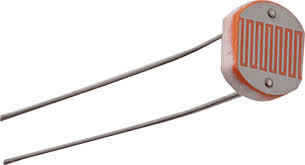
\includegraphics[scale = 0.4]{Labos-Complements/Lab09/LabDD/Figures/photoresistance.jpg}
    \caption{Exemple de photorésistance}
    \label{fig:enter-label}
\end{figure}
\subsection{Photodiodes}
Les Photodiodes agissent à la fois comme une diode standard et comme une source de courant, contrôlée par la lumière incidente. Les photons entrant en collisions avec des électrons dans les matériaux de la photodiode ont une chance d'exciter un de ceux-ci. Cette excitation créera une paire de charges libres, de signes opposées qui se «déplaceront» dans des directions opposées, dû au champ électrique intrinsèque à la photodiode. Ainsi, un courant est généré. Ce fonctionnement simplifié est celui à la base des receveurs de télécommunications, de plusieurs capteurs lumineux et des panneaux solaires.
\begin{figure}[h]
    \centering
    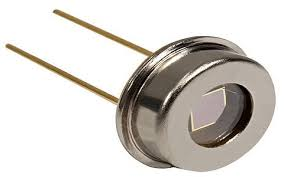
\includegraphics[scale=0.4]{Labos-Complements/Lab09/LabDD/Figures/photodiode.jpg}
    \caption{Exemple de photodiode}
    \label{fig:enter-label}
\end{figure}

\subsection{Phototransistors}

Un phototransistor fonctionne comme un transistor standard, à l'exception que la base est contrôlée par la lumière. La quantité de lumière est directement liée au signal pouvant être transmis entre le collecteur et l'émetteur. Le phototransistor peut aussi être vu comme une photodiode avec amplification. De plus, si le collecteur est laissé débranché, le phototransistor agit exactement comme une photodiode avec les deux autres terminaisons.

\begin{figure}[h]
    \centering
    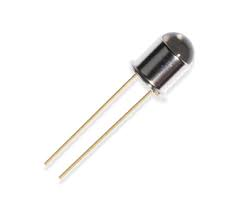
\includegraphics[scale = 0.6]{Labos-Complements/Lab09/LabDD/Figures/phototransistor.jpg}
    \caption{Exemple de phototransistor}
    \label{fig:enter-label}
\end{figure}
\newpage
\subsection{Détecteurs CCD, CMOS et EMCCD}
Ces trois termes réfèrent aux types de capteurs dans les caméras digitales commerciales et scientifiques. Les trois sont une matrice de composants photosensibles. Les capteurs CCD et EMCCD contiennent une photodiode par pixel. La seule différence entre les deux étant que les capteurs EMCCD multiplie les électrons excités avant de mesurer le signal. Les capteurs CMOS tant qu'à eux sont composés d'un phototransistor par pixel. L'avantage évident de ces capteurs est de pouvoir résoudre spatialement l'influx lumineux par l'ajout d'optiques en avant du capteur.



\end{document}

